\chapter{Introduction}
\label{sec:Introduction}

The discovery of neutrino oscillations shows that neutrinos are massive \cite{Nustatus}, which is unambiguous evidence for physics beyond the Standard Model (SM). Many extensions of the SM have been proposed so far, among which the seesaw mechanism is an appealing possibility \cite{SeesawI,typeIa,typeIb,typeIe,typeIIa,typeIIb,typeIIc,typeIId,typeIIe,SeesawIII:a,Seesawinverse}. The seesaw mechanism introduces new heavy particles coupling both to leptons and to Higgs doublets, and accounts for both the neutrino masses and their smallness (six or more orders of magnitude smaller than that of the electron).

%These new heavy particles could be weak-singlet fermions (type I \cite{SeesawI,typeIa,typeIb,typeIe}); weak-triplet scalars (type II \cite{typeIIa,typeIIb,typeIIc,typeIId,typeIIe}); or weak-triplet fermions (type III \cite{SeesawIII:a}). They generate a small Majorana mass for the neutrinos, given by, in type I and type III models: $m_{\nu}=Y^T~ \mathcal{M}^{-1}~ Y ~ v^2/2$, where $Y^T$ is the transpose of the Yukawa coupling matrix between the mediators and the SM fermions, $\mathcal{M}$ is the mass matrix of the heavy partner of the neutrinos and $~v$ is the Higgs vacuum expectation value. When mediator mass is large enough (of order of $10^{14}\,\GeV$), small neutrino masses are generated even for order $O(1)$ Yukawa couplings. If $M$ is smaller (of the order of a few hundreds of \GeV, as in LHC searches), either smaller Yukawa couplings (i.\,e. ``natural'' mixing angles of the order of $10^{-6}$) are required to generate small neutrino masses, or an alternative suppression mechanism is needed (e.\,g. seesaw inverse mechanism \cite{Seesawinverse}). The possible allowed values of the mixing parameters and their products are constrained by precision electroweak data \cite{typeIIIconstraint}.

Within the type-III seesaw model \cite{SeesawIII:a}, the neutrino is considered a Majorana particle whose mass arises via the mediation of massive fermion partners. These massive partners are the fermionic $SU(2)$ triplet of the heavy Dirac charged leptons $\Sigma^\pm$, and the heavy Majorana neutral lepton $\Sigma^0$, coupling both to the leptons and to the Higgs doublets. During proton-proton collisions, the heavy fermion particles may be pair-produced through electroweak interactions in both charged-charged and charged-neutral pairs as can be seen in Fig.~\ref{fig:SeesawProduction}.

\begin{figure}[b]
\begin{center}
	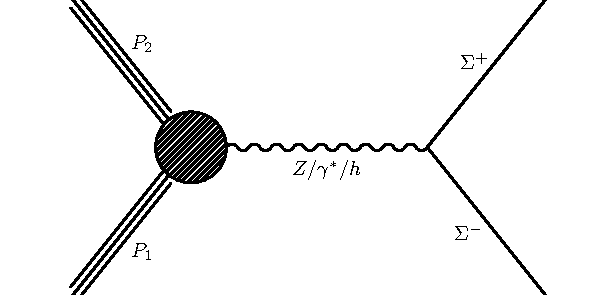
\includegraphics[width=.5\textwidth]{Introduction/SeesawProduction-SpSm}%
	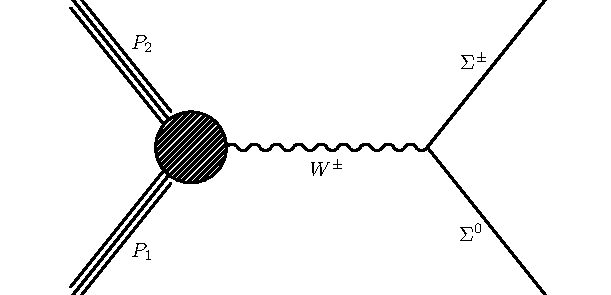
\includegraphics[width=.5\textwidth]{Introduction/SeesawProduction-SpmS0}
	\caption{Examples of Feynman diagrams for heavy fermion production in the type-III seesaw model.
	\label{fig:SeesawProduction}}
\end{center}
\end{figure}

We conduct a search for this signal by examining the final state with at least three electrons or muons. The primary decay channels of interest are $\Sigma^\pm \to \PW^\pm \nu$, $\Sigma^\pm \to \Z \ell^\pm$, $\Sigma^\pm \to \PH \ell^\pm$, $\Sigma^0 \to \PW^\pm \ell^\mp$, $\Sigma^0 \to \Z \nu$, $\Sigma^0 \to \PH \nu$, where $\ell = e, \mu$. Decays of $\Sigma^0 \Sigma^\pm$ and $\Sigma^+ \Sigma^-$ pairs result in 27 different production processes and can naturally lead to multilepton final states if several \PW\ or \Z\ bosons are involved, either directly or via a Higgs boson decay. An example Feynman diagram for one of the most relevant processes with three leptons in the final state, $\Sigma^\pm \Sigma^0 \to \PW^\pm \nu \PW^\pm \ell^\mp$ with leptonic $\PW^\pm$ decays, is shown in Fig.~\ref{fig:SeesawDecay}.
The decay rate of a $\Sigma$ to a given lepton $\ell$ is proportional to $v_{\ell N} = \frac{V_\ell}{\sqrt{|V_e|^2 + |V_\mu|^2 + |V_\tau|^2}}$. In the democratic scenario, the mixing parameters $V_\ell$ are the same for all the leptons.
%Further details on the signal phenomenology and generation can be found in Sec.~\ref{sec:Samples/Signal}.

\begin{figure}[t]
\begin{center}
	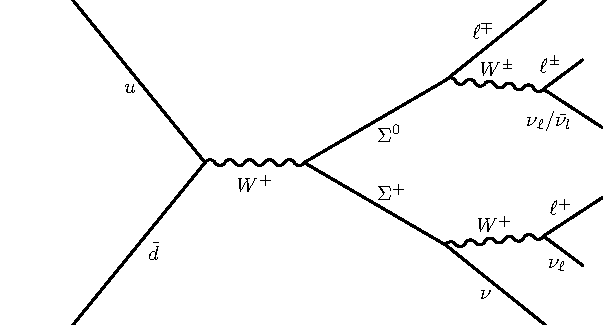
\includegraphics[width=.5\textwidth]{Introduction/Seesaw}
	\caption{Feynman diagram example of the fermion production and decay in the type-III seesaw model.
	\label{fig:SeesawDecay}}
\end{center}
\end{figure}

Prior results for this model include the EXO-14-001 PAS \cite{CMS-PAS-EXO-14-001} which set exclusion limits for the democratic scenario at $m_\Sigma = 250\,\GeV$ (expected) and $m_\Sigma = 278\,\GeV$ (observed) based on trilepton channels, and an ATLAS result in the $\ell\ell jj$ final state \cite{ATLAS-CERN-PH-EP-2015-094} which extends to higher mass values, but cannot be directly compared because of different choices of mixing parameters and other model constraints. Both these results use 8\,\TeV datasets with an integrated luminosity of 20\fbinv, whereas an older CMS result uses a 7\,\TeV dataset with 4.9\fbinv \cite{CMS-PAPER-EXO-11-073}.

Going from 8\,\TeV to 13\,\TeV, the signal cross section has increased by a factor of 3 for masses at the sensitivity limit between 300 and 400\,\GeV. Still, due to various analysis improvements which include new decay modes involving the Higgs boson, 4-lepton channels, new kinematic binning, and refined background methods, the sensitivity with the current \fullLumi dataset at 13\,\TeV exceeds that of the Run I analysis.

We pursue a broad search in final states with at least three isolated prompt leptons ($e$, $\mu$). The most notable backgrounds are \WZ decaying to three leptons, fully leptonic \ttbar decays with a misidentified\footnote{Note that the term ``misidentified'' may refer both to real leptons that arise from non-prompt decays of hadrons, for instance, and to non-leptonic objects that are reconstructed as leptons.} lepton from a b-jet, leptonic \Z decays accompanied by a misidentified lepton usually from a jet, and leptonic \ZZ decays. In addition to these, there are rare backgrounds such as $\ttbar\Z$, $\ttbar\PW$, triboson, and Higgs production.

The $VV$ backgrounds are generally well modeled by Monte Carlo (MC) simulation ($V = \PW, \Z$). Backgrounds with misidentified leptons, however, are not as easily modeled by MC simulation and are thus estimated from data.

The background estimation methods employed in this search have been used extensively in various CMS Run-I publications, e.\,g. \cite{Chatrchyan:2013xsw,Chatrchyan:2014aea,Khachatryan:2014mma,Khachatryan:2014jya}.

The central feature of the CMS apparatus is a superconducting solenoid of 6\unit{m} internal diameter, providing a magnetic field of 3.8\unit{T}. Within the superconducting solenoid volume are a silicon pixel and strip tracker, a lead tungstate crystal electromagnetic calorimeter (ECAL), and a brass and scintillator hadron calorimeter (HCAL), each composed of a barrel and two endcap sections. Forward calorimeters extend the pseudorapidity~\cite{Chatrchyan:2008zzk} coverage provided by the barrel and endcap detectors. Muons are measured in gas-ionization detectors embedded in the steel flux-return yoke outside the solenoid. A more detailed description of the CMS detector, together with a definition of the coordinate system used and the relevant kinematic variables, can be found in Ref.~\cite{Chatrchyan:2008zzk}.
